\chapter{~}
If you've never had the pleasure of waking up next to a beautiful woman in a large,
cumbersome cast after a very passionate night, you've been missing something.

Monique was already awake, and was looking at me. I was embraced with her as well as the
situation allowed: I was mostly on my stomach, one arm underneath her back and my head resting
on her shoulder. One of my legs was over one of hers. The plaster had long lost all of its
clamminess and was completely dry.

``Good morning,'' she said with a smile, and kissed me.

I smiled back. ``Yes, it IS a good morning, and it's going to be a great day.''

``Yes it is- we'd better get moving.''

Of course, she wasn't going to be doing much moving on her own today, but I would be
happily assisting her. I had a lot to do, so I got out of bed and stretched.

``Oooohhh, you're teasing me! I'd like to stretch like that,'' she said.

``Want out of it? It can happen any time you like.''

I ducked as she threw a pillow at me with a smile.

I began getting us ready. I lifted Monique out of bed, and carried her downstairs the same
way I'd carried her up the day before. Surprisingly, going downstairs was a bit trickier than
going up. Balancing and controlling the weight of two people (plus a huge plaster cast) was a
bit challenging, but it was all a part of this great adventure. Once downstairs, I carried her
to the bathroom. I was able to get her through the door by carrying her in the upright position.
By now, with the cast completely dry, I could set her down on her feet. She had to hold herself
up with one arm, but could stand up fine. I helped her answer nature's call, and then gave her a
sponge bath. We didn't wash her hair, but that was going to be taken care of later. She wanted
to do her makeup, so I turned her around to face the mirror, and went to shower and dress
myself.

When I returned, she was nearly done, so I went ahead and prepared us a light breakfast.
Once she was finished, I helped her into the black skirt and white top she'd picked out for the
day. I then lifted her into the wheelchair, and pushed her to the kitchen, where we ate as we
talked over the plans for the day. We decided to go to Cincinnati, since that was where we'd
planned to go publicking the day of the tornado. I'd set up an appointment at a nice salon
there, where she would get a haircut and anything else she wished. I'd told them that she'd been
in an accident, and was somewhat immobile. I asked if there would be any trouble with
accessibility, and they had assured me that they would be accommodating.

Lifting her into the Expedition was as difficult as it had been the day before. Not
something I want to do very often, to be sure. The drive was uneventful, she was comfortable the
whole trip, and had no issues with carsickness, despite the distance.

Arriving at the salon, I got her into the chair and wheeled her to the door. Fortunately,
it was a double door, and as we neared the door, two stylists opened the doors to meet us.

``You must be Monique.'' One of them said as I pushed her through the door. ``My goodness, he
told us you were in a bad accident, but those casts are huge! What happened to you, anyway?''

\begin{thought}
Quinn always thinks of everything, but we'd forgotten that we'd probably get questions from
people we met. Monique thought quickly then spoke:
\end{thought}

``Well, it's actually only one cast,'' she said, lifting her shirt to show some of the
plaster over her midsection.

The girl's jaw dropped. ``Oh my God, that must be terrible! I've never seen a cast so big!
What happened to you, anyway?''

``A wall collapsed on me during the tornado that went through a couple of months ago,''
Monique said. I was impressed at her ability to make up a story so quickly, and not a lame car
crash, either- she took an event that had been big news in the entire region and made her cast a
part of it.

Mesmerized or horrified, this young lady kept asking questions as we wheeled her to the
chair. It wasn't a huge salon, and wasn't packed, but there were a few other customers there,
and they all turned to get a glance at the woman in the huge cast.

``What did you break to get a body cast like that?'' She asked as she reclined the salon
chair and turned it toward us. I lifted Monique into the chair and pushed the chair aside as I
took a seat, and enjoyed the conversation between them.

``Well, when the wall collapsed on me, it broke both of my legs between the knee and ankle,
and it also broke my left leg above the knee, and both of my hips, as well,'' Monique answered.

The girl pumped the chair up as high as it would go, but still had to crouch down a bit to
get to work on Monique's hair. She worked slowly, asking more and more questions about Monique's
``injury'' and coping with life in the cast.

\begin{thought}
This was big fun for Monique. She was the center of attention of the whole shop. She
noticed the other stylists were not having the usual small talk conversations with their
clients: everyone was listening to the conversation between her and her stylist. The questions
seemed to never end, and Monique loved answering them all: ``How long do you have to wear it?''
``Does it get hot'' ``Does it itch?'' ``My goodness, just going to the rest room has to be a
chore in
that, isn't it?'' Despite the fact that she was being somewhat nosy, Monique was very pleased
with the job she'd done washing and trimming her hair.
\end{thought}

When she'd finished with her hair, the stylist asked what else Monique would like. Monique
asked for a manicure and pedicure.

``Normally, we do those in the other room, but I'll have Jolene come to you. I'll be right
back.'' She left to get the person who does the nails, and Monique motioned me over and pulled
my
ear close to her lips.

``I think we're giving them quite the show,'' she whispered.

``Definitely,'' I responded. ``Are you having fun?''

``This is great, I'm having a ball.''

``I'm going to go get my paper and pencil. I want to capture us a memory of this.'' I smiled
and kissed her, as the stylist returned with the lady who would do Monique's nails. She was an
older lady, probably in her mid 50's. I excused myself for a moment and went and retrieved my
supplies. When I returned, the lady was still sizing up exactly how to approach the work on
Monique.

``My goodness, you have hurt yourself, haven't you?'' she looked at Monique's feet. ``Hm, we
won't be able to soak them first, but I'll do the best I can.'' She carefully washed Monique's
toes with a damp rag, and actually asked the standard generic questions as she worked.

I enjoyed watching the whole scene as Monique got the first class treatment: Monique
sneaking smiles at me, the employees and the patrons looking at the ``poor lady'' in the big
cast.
By the time she was finished with her hands, her toes were already dry, and the bright red
polish looked great contrasting with the white cast. Monique definitely chose an attention
grabbing color. While she waited for the fingernail polish to dry, I drew a quick sketch of her.

When she was ready, I lifted her back into the wheelchair, paid the bill, nicely tipped the
ladies who'd worked on her and we left. The one who had done her hair told me I was a good guy
for pampering her this way, and wished Monique a speedy recovery.

Once we were back in the truck and on the road, we laughed as we recounted the experience.
The questions, the looks, the sideways sneak looks, and the outright stares- it was all a lot
more fun than we expected it to be. One thing that stuck out on a serious note- nobody expressed
any doubts as to the cover story or the cast itself.

``We gotta go have some more fun with this thing.'' Monique said. ``Where to next?''

``Let's get something to eat.'' I answered. ``No drive through, either- someplace nice and
public.''

She agreed, and we started watching for suitable places. Soon, we found ourselves in an
interesting looking area. Though clearly in an older section of downtown, everything was clean
and well kept, and the businesses suggested that this was probably one of the trendy places.
More importantly, the sidewalks were quite busy with a lot of pedestrian traffic. Soon, we
spotted a restaurant that had a garden dining area near the street. I looked at Monique and she
nodded without a word.

I found us a parking place a couple of blocks away. I passed a couple of open spots getting
to it, but I wanted to wheel my ``badly injured'' beauty through the people walking along the
street, and we were quite the spectacle as we made our way to the café'. At least Monique was
quite the spectacle.

The outdoor dining garden was a couple of feet below street level. Fortunately, there was a
ramp. It's odd that accessibility features barely capture our notice if we have no need for
them. We see them, but they barely register in our minds. However, when you NEED them, you spot
them from quite a distance, and are very happy to see them.

As the hostess approached us, she did a slight double take at Monique, and then snapped
back to being professional. We asked for a table for two, and she led us to an open table that
had a nice view. In truth, it had two nice views: we were next to a fountain rimmed with
flowerbeds, and we were easily open to the street. Along the way to the table, I noticed people
looking at us. Some were very discreet, and a few just outright stared as we passed them. The
hostess pulled the chair out of the way so I could wheel Monique close to the table, then
stopped and turned to us.

``Will this table be alright, or would you like something more private?'' I think she was
offering us the chance to be less conspicuous. I suppose that was nice, but even if Monique were
truly injured, we wouldn't be out in such a busy area if we didn't want to be seen.

``No, this is great,'' Monique answered her. She smiled and left to send our waitress to us.

The waitress was very professional. Either Monique's cast didn't faze her, or, more likely,
the hostess had already told her about it. She took our order and left us.

While we waited for our food, we chatted. We mostly chatted quietly about some of the
people sitting nearby, and the ones walking by along the sidewalk. Most of them seemed a bit
startled when they first saw Monique, but then returned to their conversations, and paid us no
further attention.

One couple, however, was different. They were a middle aged couple. They were dressed
neatly, but casually. They were seated across the garden to my right, and Monique's left. As we
entered, we'd clearly caught their eye. While we waited, they seemed to look our way somewhat
frequently. Perhaps we were being a bit self-interested but it seemed to Monique and I that we
(or Monique, actually) had become the topic of their conversation.

By the time our food arrived, they were finishing theirs, but they stayed while we ate.
Perhaps if he'd been alone, or if they'd looked scruffy, I might have been a bit concerned. As
it was, they had an upper middle class appearance about them.

As we ate, our conversation turned to ideas for what to do with the rest of the day. We'd
discussed finding a shopping mall to ``show off'' in, but over lunch, we decided to stay in this
area and explore some of the shops in the area, and decide later if we wanted to go to a mall or
not.

``Excuse me $\ldots$'' I hadn't noticed the middle aged couple walking our way. Now, they were
at our
table, and the man was addressing us.

``I'm sorry to interrupt your lunch, but I couldn't help but notice your casts,'' he said to
Monique. He seemed slightly nervous as he asked, or maybe that was my imagination.

``I can't help but notice, either.'' Monique said with a smile. ``Hi, I'm Monique, and this is
Quinn,'' she added as she nodded my direction.

``I'm Dave,'' the man answered, smiling at Monique's remark. ``And this is my wife Molly.'' He
turned back to Monique. ``I didn't mean to stare, and I am very sorry if we bothered you. I used
to be an orthopedic technician, and leg casts attached with a spreader bar are extremely rare.
In fact, I've never seen them on an adult, except in books on the history of orthopedics.''

\newpage
\begin{center}
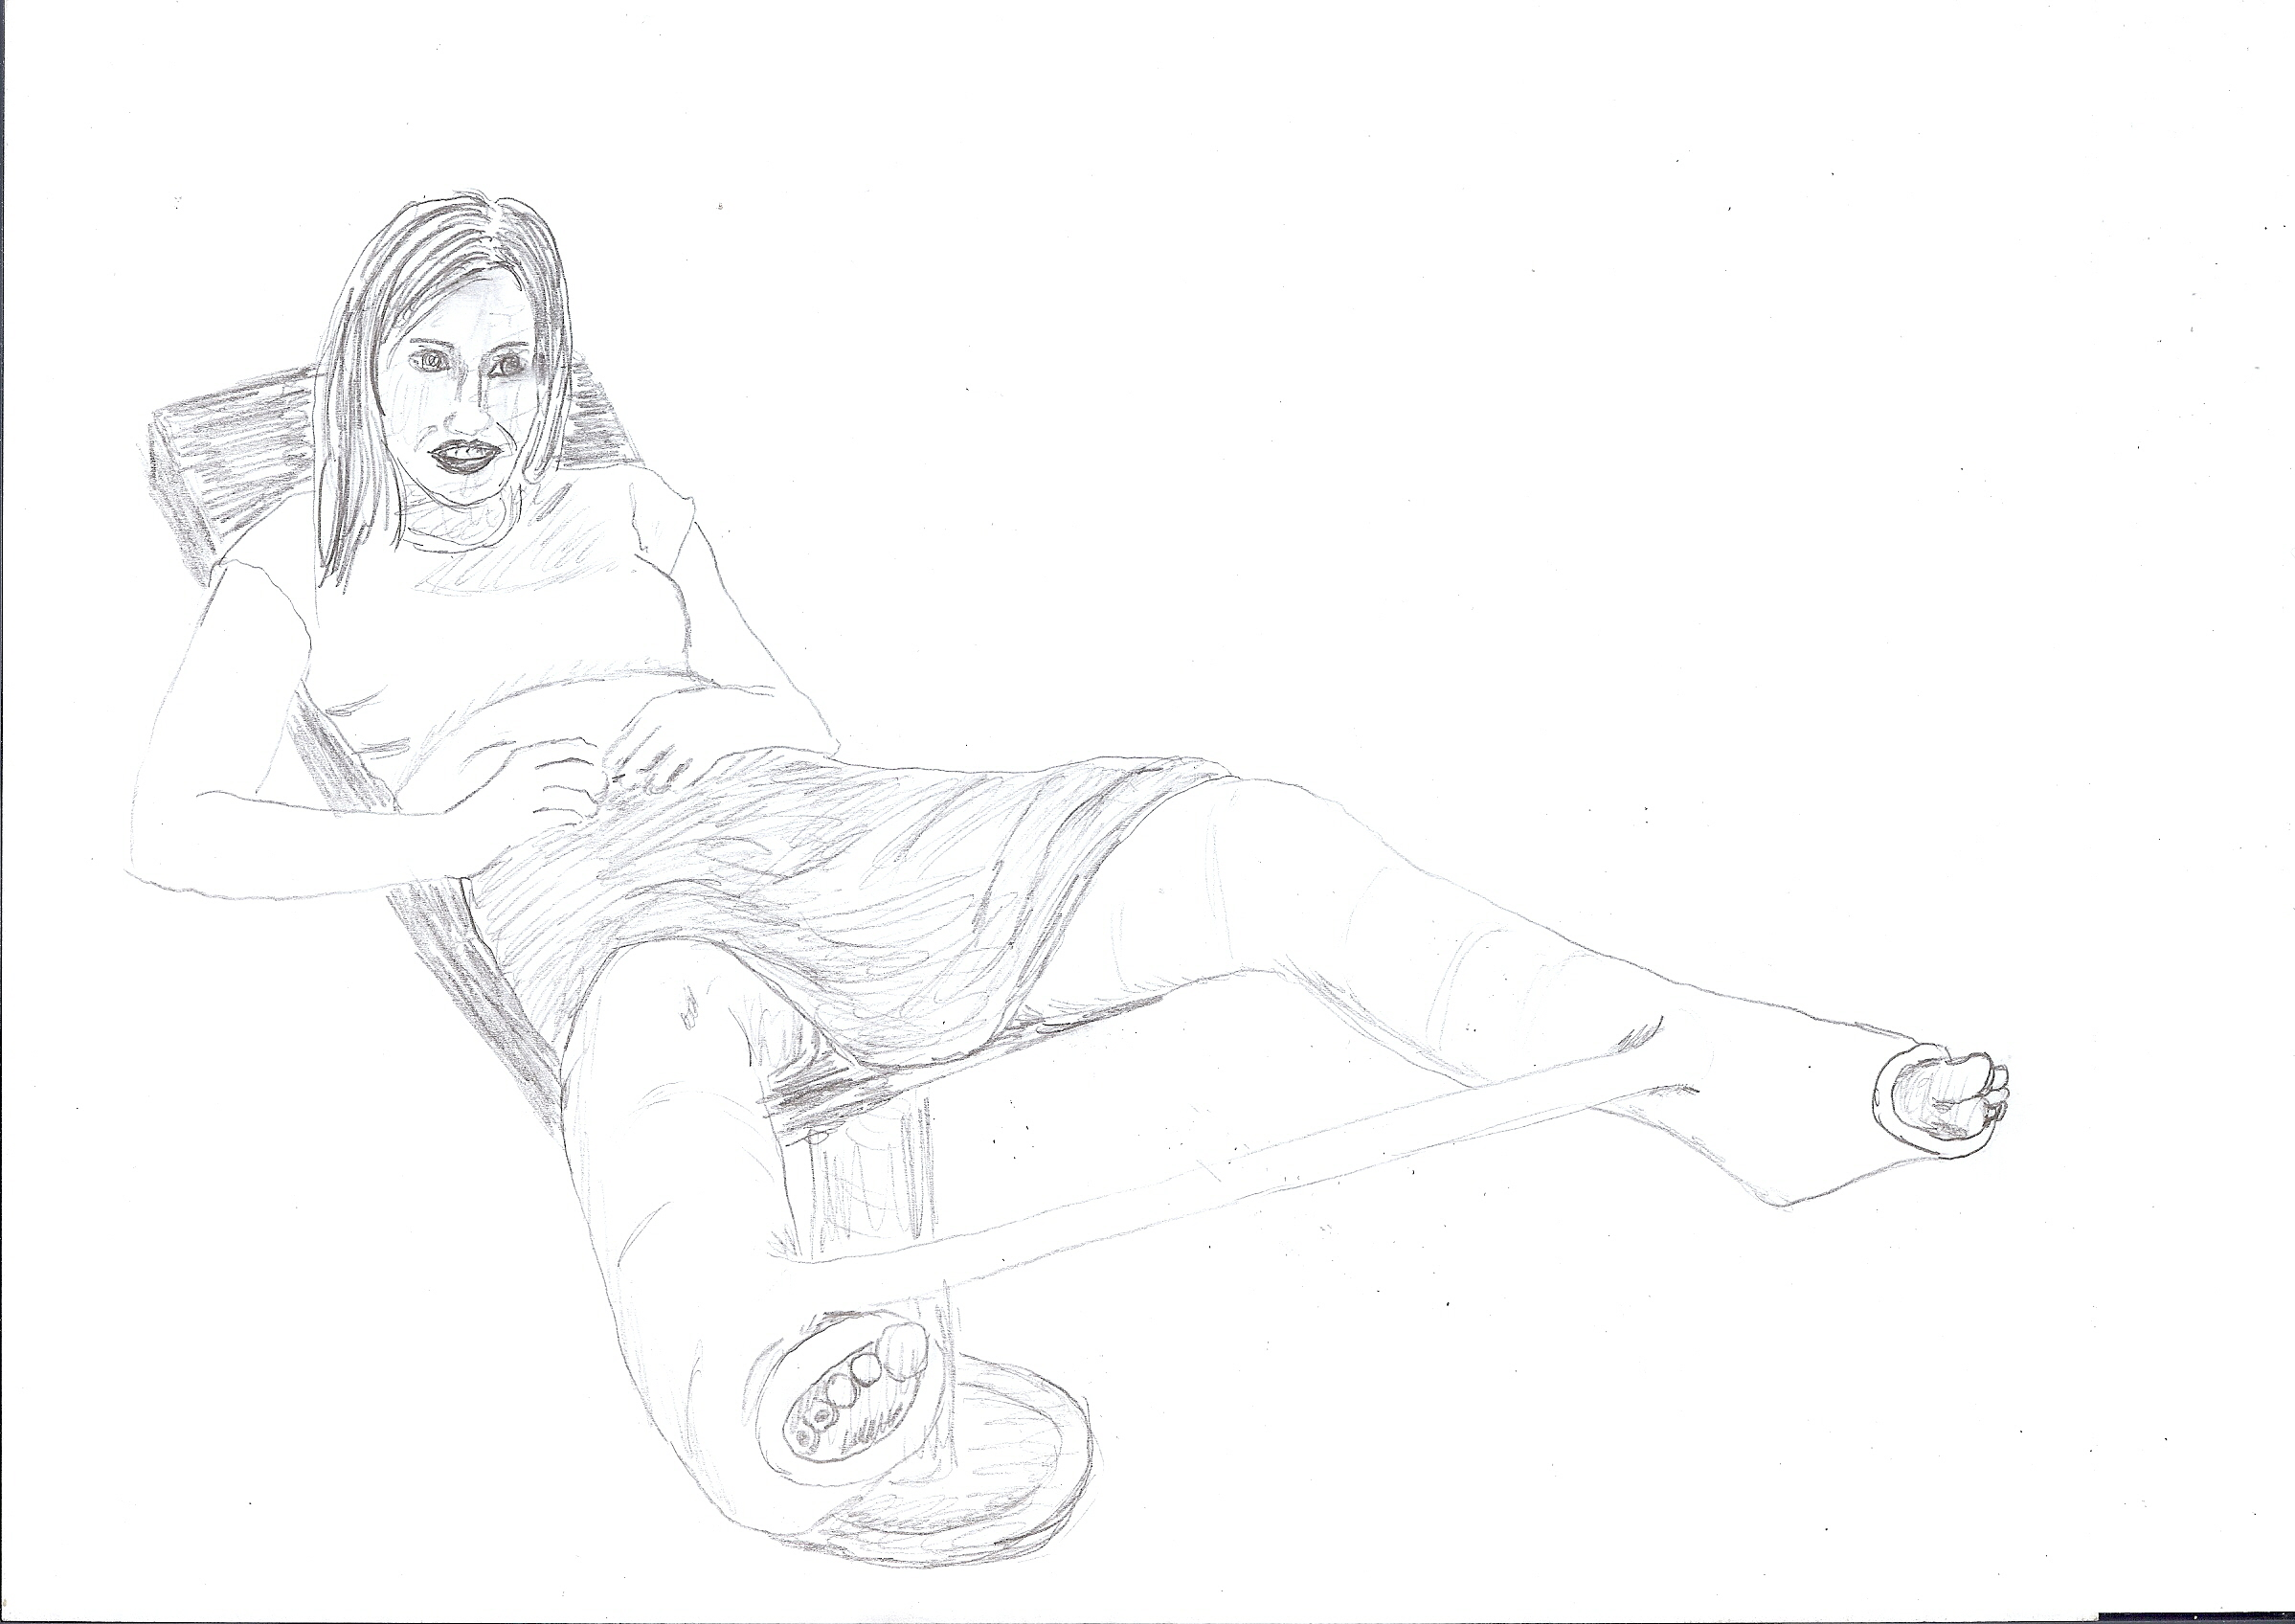
\includegraphics[width=\textwidth]{images/kicks43.jpg}
\end{center}
